\section{Uvod}
\subsection{Raspberry pie}
Raspberry pie je serija malih "single-board" računala široko korištenih u svrhe eksperimentalnih projekata.
\paraBreak
Idealan je za tu upotrebu zbog privlačne cijene i odlične portabilnosti te jako male potrošnje struje.
\paraBreak
Za ovaj rad je odabran zbog osim navedenih razloga još i radi ogromnog izbora eksternih modula, specifično službenog kamera modula
koji služi kao baza cijelog projekta.

\begin{figure}[ht]
  \centering
  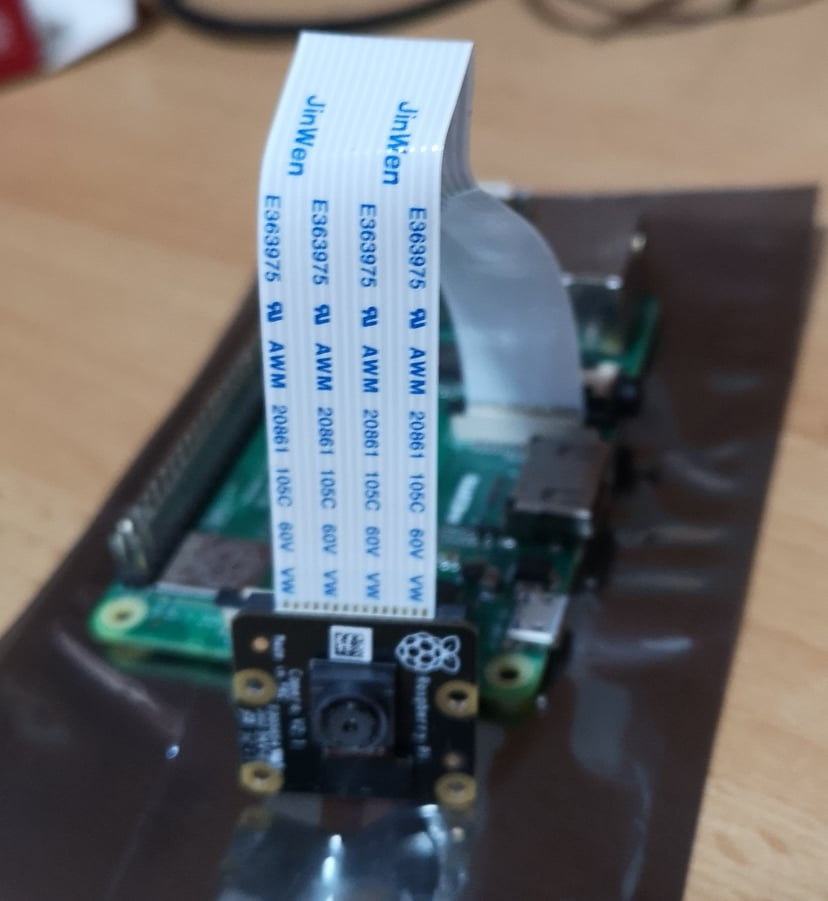
\includegraphics[width=0.6\textwidth]{raspberyy-pi-camera.jpg}
  \caption{Raspberry pi kamera modul}
\end{figure}

\begin{figure}[ht]
  \centering
  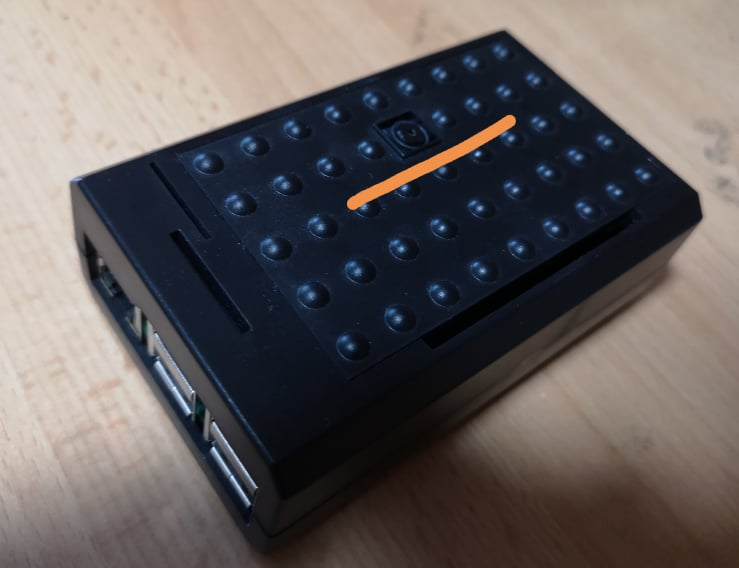
\includegraphics[width=\textwidth]{raspberyy-pie-in-box.jpg}
  \caption{Raspberry pi u kutiji sa otvorom za leću kamere}
\end{figure}

\clearpage
\subsection{FFmpeg}
FFmpeg je open-source projekt koji se sastoji od mnoštva biblioteka za manipuliranje videom, audiom i ostalom multimedijom.
\paraBreak
Najveća primjena mu je u transkodiranju, editiranju, skaliranju i raznim efektima videa.
\paraBreak
Najbitnije biblioteke iz FFmpeg-a koje se koriste u ovom radu su
\begin{itemize}
  \item libavcodec - audio/video kodek biblioteka
  \item libavformat - audio/video kontejner mux i demux biblioteka (više u daljnim poglavljima)
  \item libavdevice - biblioteka za dohvačanje i rad dostupnim multimedija uređajima
  \item libavscale - biblioteka za manipulaciju i skaliranje slika videa
\end{itemize}
Koristi se u mnogim popularnim projektima kao što su Google Chrome, VLC Player, Youtube, Blender, Handbrake, Kodi, Plex.
